
\documentclass[12pt,a4paper]{ctexart}

\usepackage[a4paper,margin=2.4cm]{geometry}
\usepackage{array}
\usepackage{booktabs}
\usepackage{enumitem}
\usepackage{hyperref}
\usepackage{longtable}
\usepackage{setspace}
\usepackage{graphicx}
\usepackage{xcolor}
\usepackage{listings}
\usepackage{float}
\usepackage{caption}
\usepackage{subcaption}
\usepackage{fancyhdr}
\usepackage{tikz}
\usepackage{amssymb}
\usetikzlibrary{shapes.geometric, arrows, positioning, fit, backgrounds}

\hypersetup{
  colorlinks=true,
  linkcolor=black,
  urlcolor=blue,
  pdftitle={操作系统课程设计A题结题报告},
  pdfauthor={侯奕明, 涂凡琛, 韩硕}
}

\setstretch{1.3}
\setlist[itemize]{leftmargin=2em}
\setlist[enumerate]{leftmargin=2.2em}
\ctexset{
  section = {
    format = \Large\bfseries,
    number = \chinese{section}、
  },
  subsection = {
    format = \large\bfseries,
    number = \arabic{section}.\arabic{subsection}
  },
  subsubsection = {
    format = \bfseries,
    number = \arabic{section}.\arabic{subsection}.\arabic{subsubsection}
  }
}

% 代码样式
\lstset{
  basicstyle=\small\ttfamily,
  breaklines=true,
  frame=single,
  numbers=left,
  numberstyle=\tiny,
  tabsize=2,
  language=C,
  showstringspaces=false
}

\title{\textbf{《操作系统课程设计》A题结题报告}}
\author{侯奕明 \quad 涂凡琛 \quad 韩硕}
\date{2026年6月}

\begin{document}

\begin{titlepage}
  \centering
  \vspace*{3.5cm}

  {\zihao{2}\bfseries 《操作系统课程设计》A题结题报告\par}
  \vspace{1.2cm}
  {\zihao{4}项目题目：OS 内核实现\par}
  \vspace{0.6cm}
  {\zihao{4}基础平台：xv6-riscv\par}
  \vspace{1.6cm}

  \renewcommand{\arraystretch}{1.5}
  \begin{tabular}{>{\bfseries}p{3.2cm}p{8.5cm}}
    课程名称   & 操作系统课程设计 \\
    报告性质   & 结题报告（方案A） \\
    小组成员   & 侯奕明、涂凡琛、韩硕 \\
    当前选题   & A题：OS 内核实现 \\
    提交时间   & 2026年6月 \\
  \end{tabular}

  \vfill
  {\large \today\par}
\end{titlepage}

\tableofcontents
\newpage

%=====================================================================
\section{项目概述}
%=====================================================================

\subsection{项目背景}

操作系统是计算机系统的核心软件，负责管理硬件资源、提供程序运行环境。本课程设计要求学生基于 xv6-riscv 教学操作系统，深入理解并扩展操作系统内核的核心功能。xv6 是由 MIT 开发的教学操作系统，最初基于 x86 架构，后移植到 RISC-V 架构。xv6-riscv 包含了操作系统最基本的功能模块：系统启动、中断与异常处理、内存管理、进程管理、文件系统以及用户程序加载与执行，是学习操作系统内核实现的理想平台。

本项目选择《操作系统课程设计》项目制方案中的\textbf{A 题"OS 内核实现"}，以 xv6-riscv 为基础平台，围绕系统调用接口、中断与异常处理、设备驱动、进程管理、内存管理、文件系统以及网络协议栈等核心模块展开，在成功复现和理解现有系统的基础上，完成了课程要求的各项功能，并在此之上进行了大量扩展创新。

\subsection{项目目标}

本项目的核心目标是：

\begin{enumerate}
  \item 成功复现 xv6-riscv 的运行环境，理解其启动流程与整体架构；
  \item 按照 A 题六大模块要求，逐项完成功能实现与验证；
  \item 在基础功能之上进行创新扩展，包括但不限于：新增系统调用、网络协议栈、调度算法优化、内核堆分配器等；
  \item 完成完整的测试验证，确保系统稳定运行；
  \item 形成规范的技术文档，为后续学习者提供参考。
\end{enumerate}

\subsection{团队信息与分工方案}

本组共三名成员，按照 A 题六大模块进行分工，各自负责核心模块的分析、实现与文档工作。

\begin{table}[H]
\centering
\caption{小组成员与分工}
\begin{tabular}{>{\bfseries}p{2.5cm}p{4.5cm}p{6cm}}
\toprule
\textbf{成员} & \textbf{负责模块} & \textbf{主要工作内容} \\
\midrule
侯奕明 & 接口、设备与软件交互 & 系统调用接口（ps/halt/lseek/socket）、trap路径、控制台/串口驱动、virtio-net网卡驱动、UDP协议栈、Shell功能增强 \\
\hline
涂凡琛 & 进程管理与处理机调度 & FCFS/MLFQ/RR调度算法、信号量机制、wakeup哈希队列优化、调度测试程序 \\
\hline
韩硕 & 内存管理与文件系统 & 内核堆分配器（kmalloc/kmfree）、页表管理、文件描述符表管理、文件系统各模块分析 \\
\bottomrule
\end{tabular}
\end{table}

此外，整个小组共同承担了以下工作：
\begin{itemize}
  \item xv6 项目的整体框架搭建与环境配置；
  \item QEMU 运行验证与基础调试；
  \item 模块间联调与问题定位；
  \item 课程进度报告、结题报告和汇报材料整理。
\end{itemize}

\subsection{项目完成情况概览}

截至结题阶段，本组已完成的工作包括：

\begin{table}[H]
\centering
\caption{项目完成情况总览}
\begin{tabular}{>{\bfseries}p{4cm}p{3cm}p{3cm}p{3cm}}
\toprule
\textbf{功能模块} & \textbf{基础功能} & \textbf{扩展功能} & \textbf{测试状态} \\
\midrule
系统启动与初始化       & 已完成 & --    & $\checkmark$ 通过 \\
中断与异常处理         & 已完成 & --    & $\checkmark$ 通过 \\
系统调用接口           & 已完成 & 新增4个 & $\checkmark$ 通过 \\
设备驱动（UART/virtio）& 已完成 & virtio-net & $\checkmark$ 通过 \\
控制台I/O             & 已完成 & 输出原子化 & $\checkmark$ 通过 \\
Shell功能增强          & 已完成 & PATH fallback/halt内置 & $\checkmark$ 通过 \\
进程管理与调度         & 已完成 & FCFS/MLFQ & $\checkmark$ 通过 \\
信号量机制             & 已完成 & 3组测试 & $\checkmark$ 通过 \\
内存管理               & 已完成 & kmalloc堆分配器 & $\checkmark$ 通过 \\
文件系统               & 已完成 & lseek/文件描述符管理 & $\checkmark$ 通过 \\
网络协议栈（UDP）      & 新增   & 全协议栈 & $\checkmark$ 通过 \\
wakeup哈希队列优化     & 已完成 & O(N)→O(k) & $\checkmark$ 通过 \\
\bottomrule
\end{tabular}
\end{table}

\newpage

%=====================================================================
\section{技术方案设计}
%=====================================================================

\subsection{整体架构}

本项目的技术路线是以 xv6-riscv 为基础实验平台，结合课程 A 题要求完成三步工作：复现验证现有功能、补齐缺失功能、创新扩展新功能。整体系统架构如图\ref{fig:arch}所示。

\begin{figure}[H]
\centering
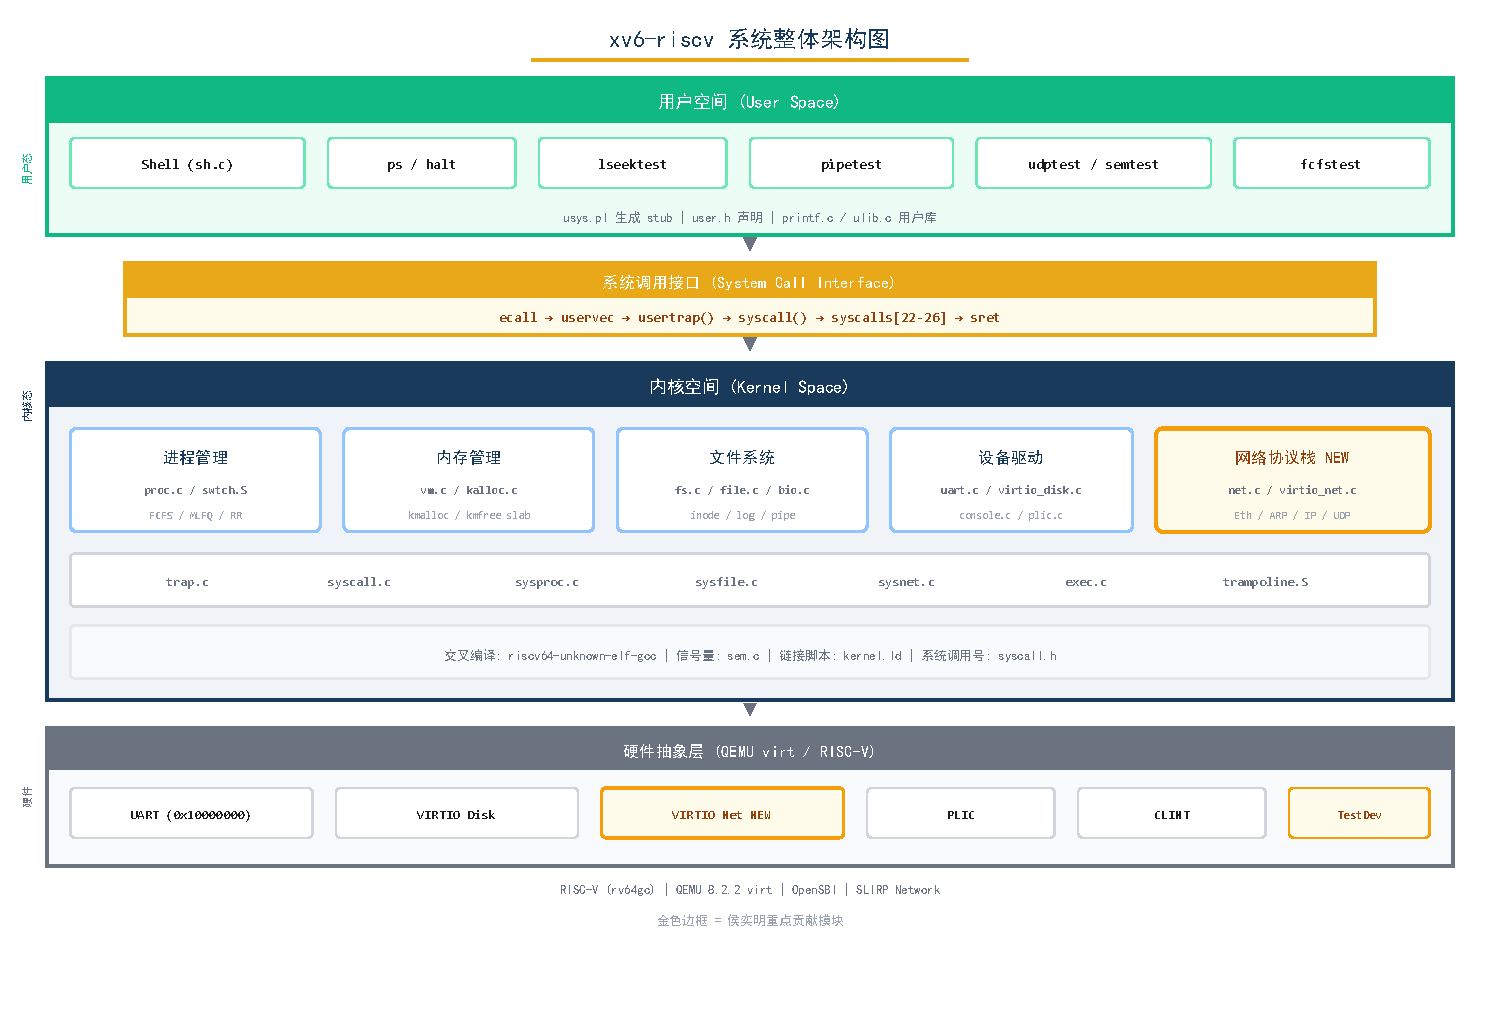
\includegraphics[width=\textwidth]{images/fig1_system_arch.pdf}
\caption{系统整体架构图}
\label{fig:arch}
\end{figure}

\subsection{模块划分}

系统从功能角度划分为以下核心模块：

\begin{enumerate}
  \item \textbf{系统启动模块}：从 M-mode 到 S-mode 的切换、内核初始化、第一个用户进程创建；
  \item \textbf{中断与异常处理模块}：trap 入口设置、系统调用分发、时钟中断、设备中断、缺页异常处理；
  \item \textbf{系统调用接口模块}：系统调用注册、参数传递、返回值处理、新增系统调用；
  \item \textbf{设备驱动模块}：UART 串口驱动、virtio 磁盘驱动、virtio-net 网卡驱动、PLIC 中断控制器；
  \item \textbf{进程管理模块}：进程生命周期、调度算法（RR/FCFS/MLFQ）、信号量同步；
  \item \textbf{内存管理模块}：页级分配器（kalloc）、内核堆分配器（kmalloc）、页表管理；
  \item \textbf{文件系统模块}：inode 层、目录与路径解析、文件描述符管理、lseek；
  \item \textbf{网络协议栈模块}：Ethernet/ARP/IP/UDP 四层协议、socket 系统调用接口。
\end{enumerate}

\subsection{技术选型}

\begin{table}[H]
\centering
\caption{技术选型说明}
\begin{tabular}{>{\bfseries}p{3.5cm}p{9.5cm}}
\toprule
\textbf{技术项} & \textbf{选择与理由} \\
\midrule
指令集架构   & RISC-V（rv64gc）：开源、简洁、现代，xv6 原生支持 \\
模拟平台     & QEMU 8.2.2（virt 机器）：完整的 RISC-V 系统模拟，支持 MMIO 设备 \\
内核基座     & xv6-riscv：MIT 教学内核，代码精简（约8000行），适合学习与扩展 \\
编译器       & riscv64-unknown-elf-gcc：RISC-V 交叉编译工具链 \\
构建系统     & GNU Make + Perl（usys.pl 自动生成系统调用 stub） \\
网络设备     & virtio-net MMIO：相比 E1000 PCIe 在 QEMU RISC-V 上更稳定（避免 PCIe DMA bug） \\
调度算法     & 编译期宏选择（SCHED\_RR / SCHED\_FCFS / SCHED\_MLFQ），避免运行时开销 \\
内存分配     & 两级架构：kalloc（4KB页）+ kmalloc（slab小对象 + 大对象回退） \\
\bottomrule
\end{tabular}
\end{table}

\newpage

%=====================================================================
\section{模块详细实现}
%=====================================================================

本章按照分工详细描述各模块的设计思路、数据结构、关键算法和核心代码实现。
其中第3.1至3.5节为侯奕明负责部分（重点），第3.6节为涂凡琛负责部分，第3.7节为韩硕负责部分。

%---------------------------------------------------------------------
\subsection{中断与异常处理（侯奕明）}
%---------------------------------------------------------------------

\subsubsection{设计思路}

中断与异常处理是操作系统的核心机制，负责管理系统调用（ecall）、时钟中断、设备中断和缺页异常。我（侯奕明）负责对该模块进行全面分析和实现，重点包括：

\begin{itemize}
  \item 系统调用全链路：从用户态 ecall 到内核 syscall 分发再到 sret 返回的完整路径；
  \item 中断处理的两条路径：用户态被中断（uservec→usertrap）vs 内核态被中断（kernelvec→kerneltrap）；
  \item 时钟中断与调度触发点（yield）；
  \item 控制台 I/O 的中断驱动数据流。
\end{itemize}

\subsubsection{系统调用全链路}

一次系统调用的完整生命周期是理解用户态与内核态交互的核心。以 \texttt{write(1, "hello", 5)} 为例，其完整路径如下：

\begin{enumerate}
  \item \textbf{用户态准备}：用户程序调用 \texttt{write()} → \texttt{user/usys.pl} 生成的汇编 stub 执行 \texttt{li a7, SYS\_write; ecall; ret}
  \item \textbf{硬件陷入}：ecall 指令触发 trap，CPU 硬件将 \texttt{scause} 设为 8（Environment call from U-mode），\texttt{sepc} 设为 ecall 指令地址，\texttt{stvec} 指向 trampoline 页中的 \texttt{uservec}
  \item \textbf{上下文保存}：\texttt{trampoline.S:uservec} 保存全部 32 个通用寄存器到 trapframe，切换页表（用户页表→内核页表），跳转到 \texttt{usertrap()}
  \item \textbf{Trap 分发}：\texttt{trap.c:usertrap()} 检查 \texttt{scause}：
    \begin{itemize}
      \item \texttt{scause == 8}：系统调用 → 调用 \texttt{syscall()}
      \item \texttt{scause == 13/15}：缺页异常 → 调用 \texttt{vmfault()}
      \item \texttt{scause \& 0x8000000000000000}：中断 → 调用 \texttt{devintr()}
    \end{itemize}
  \item \textbf{系统调用分发}：\texttt{syscall.c:syscall()} 从 \texttt{trapframe->a7} 取系统调用号，查 \texttt{syscalls[]} 表，调用对应 \texttt{sys\_write()}，返回值写入 \texttt{trapframe->a0}
  \item \textbf{返回准备}：\texttt{trap.c:prepare\_return()} 关中断，设置 \texttt{stvec=uservec}（为下次用户态 trap 做准备），设置 SPP=0（让 sret 回到 U-mode）、SPIE=1（回到用户态后开中断）
  \item \textbf{恢复现场}：\texttt{trampoline.S:userret} 从 trapframe 恢复全部寄存器，切回用户页表，执行 \texttt{sret}
\end{enumerate}

\begin{figure}[H]
\centering
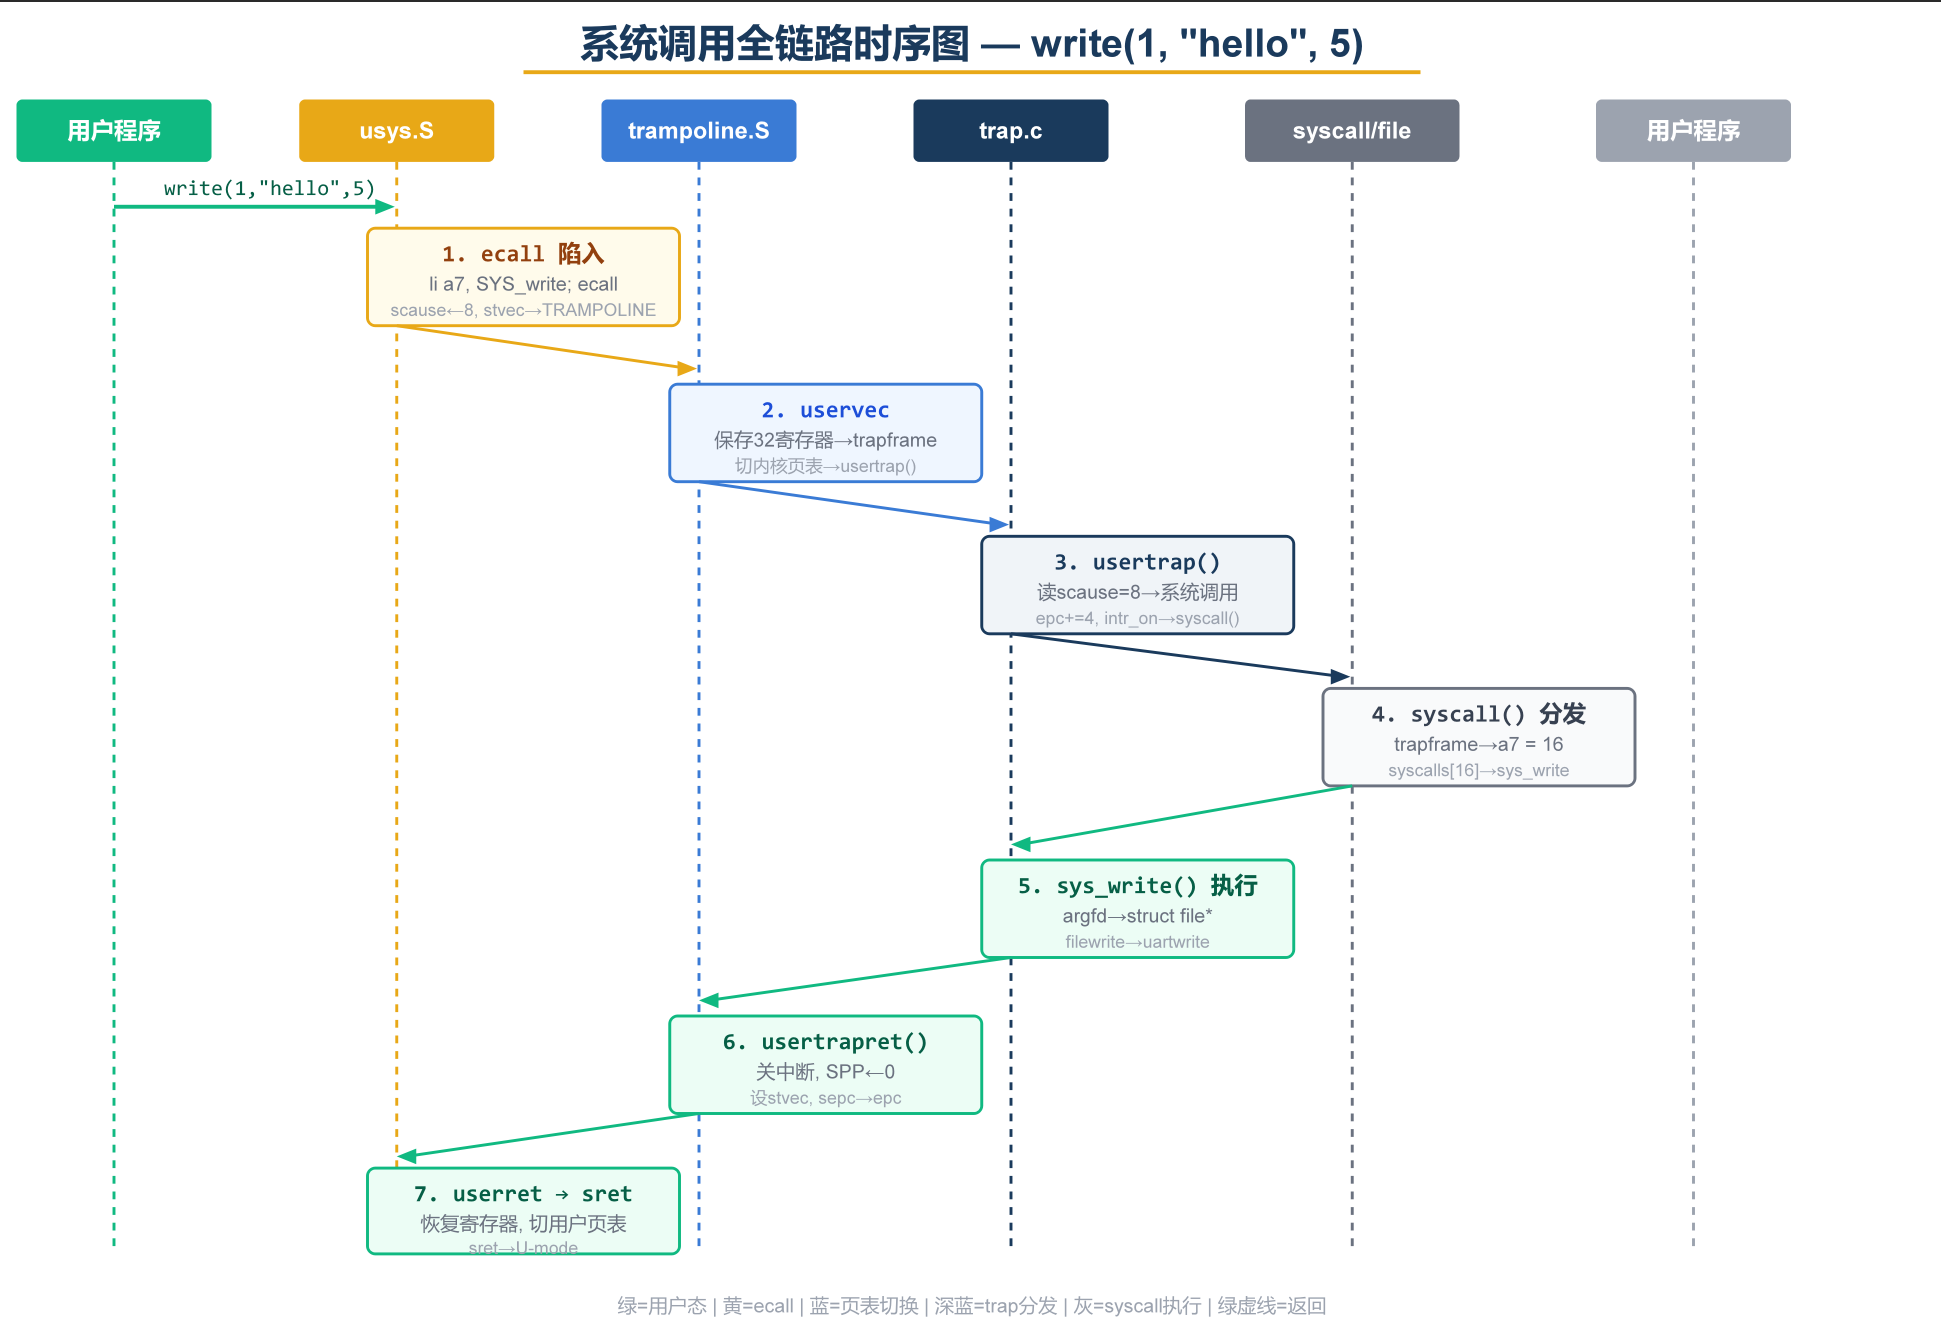
\includegraphics[width=\textwidth]{images/fig2_syscall_timing.png}
\caption{系统调用全链路时序图}
\label{fig:syscall-path}
\end{figure}

\subsubsection{中断处理的两条路径}

中断处理根据被中断时的特权级分为两条路径：

\textbf{路径A：用户态被中断}

\begin{flushleft}
\small\ttfamily
用户进程运行中                                          \\
~~$\rightarrow$ 时钟/设备中断触发                         \\
~~~~$\rightarrow$ uservec (trampoline.S) 保存寄存器、切内核页表 \\
~~~~~~$\rightarrow$ usertrap() 分发：                     \\
~~~~~~~~$\rightarrow$ devintr() 判断中断类型：              \\
~~~~~~~~~~$\cdot$ scause=0x8000000000000005 $\rightarrow$ clockintr() $\rightarrow$ 返回 2 \\
~~~~~~~~~~$\cdot$ scause=0x8000000000000009 $\rightarrow$ plic\_claim() $\rightarrow$ 设备处理 \\
~~~~~~~~$\rightarrow$ which\_dev==2 则 yield()（时间片调度触发点） \\
~~~~~~$\rightarrow$ prepare\_return() 准备返回用户态         \\
~~~~$\rightarrow$ userret (trampoline.S) 恢复寄存器、sret   \\
~~$\rightarrow$ 回到用户态继续执行
\end{flushleft}

\textbf{路径B：内核态被中断}

\begin{flushleft}
\small\ttfamily
内核代码运行中                                          \\
~~$\rightarrow$ 时钟/设备中断触发                         \\
~~~~$\rightarrow$ kernelvec (kernelvec.S) 保存寄存器       \\
~~~~~~$\rightarrow$ kerneltrap() 处理：                    \\
~~~~~~~~$\rightarrow$ devintr() 同样判断中断类型             \\
~~~~~~~~$\rightarrow$ which\_dev==2 则 yield()              \\
~~~~~~$\rightarrow$ 恢复 sepc/sstatus                       \\
~~~~$\rightarrow$ sret 回到内核继续执行
\end{flushleft}

\textbf{关键代码位置}：
\begin{itemize}
  \item \texttt{trap.c:85} — \texttt{if (which\_dev == 2) yield()} — 时间片调度的触发点
  \item \texttt{trap.c:187-220} — \texttt{devintr()} 的完整分流逻辑
  \item \texttt{trap.c:167-180} — \texttt{clockintr()}：ticks++、wakeup、预约下一次时钟中断
  \item \texttt{trap.c:29 vs trap.c:112} — \texttt{stvec} 在内核态 vs 回用户态前的切换
\end{itemize}

\subsubsection{时钟中断机制}

\begin{lstlisting}[language=C, caption={clockintr() — 时钟中断处理（kernel/trap.c:167-180）}]
void clockintr() {
  // 递增系统时钟计数
  ticks++;

  // 唤醒所有等待时钟的进程（如 pause()）
  wakeup(&ticks);

  // 预约下一次时钟中断（约10ms后，即约100Hz）
  w_stimecmp(r_time() + 1000000);
}
\end{lstlisting}

时钟中断频率由 \texttt{start.c} 中的 \texttt{timerinit()} 设定，通过设置 \texttt{stimecmp} 寄存器预约第一次中断，之后每次 \texttt{clockintr()} 中预约下一次，形成约 100Hz 的稳定时钟中断流。时钟中断是时间片轮转调度、\texttt{pause()} 睡眠/唤醒等机制的基础。

%---------------------------------------------------------------------
\subsection{系统调用接口实现（侯奕明）}
%---------------------------------------------------------------------

我负责了全部新增系统调用的设计与实现，包括 \texttt{ps}（进程列表）、\texttt{halt}（关机）、\texttt{lseek}（文件定位）以及 4 个 socket 网络系统调用。

\subsubsection{ps 系统调用}

\textbf{设计动机}：xv6 原有的进程信息查看只能通过 Ctrl-P 在内核态触发 \texttt{procdump()}，用户态程序无法获取进程列表。新增 \texttt{ps} 系统调用将其暴露给用户态。

\textbf{实现策略}：零新增内核逻辑——\texttt{sys\_ps()} 直接复用 \texttt{proc.c} 中已有的 \texttt{procdump()}。

\textbf{修改文件清单}：

\begin{table}[H]
\centering
\caption{ps 系统调用修改文件}
\begin{tabular}{>{\bfseries}p{4.5cm}p{8cm}}
\toprule
\textbf{文件} & \textbf{修改内容} \\
\midrule
\texttt{kernel/syscall.h} & 新增 \texttt{\#define SYS\_ps 22} \\
\texttt{kernel/syscall.c} & 新增声明 + \texttt{syscalls[]} 表中注册 \texttt{[SYS\_ps] sys\_ps} \\
\texttt{kernel/sysproc.c} & 新增 \texttt{sys\_ps()} 函数，直接调用 \texttt{procdump()} \\
\texttt{user/usys.pl} & 新增 \texttt{entry("ps");} — 自动生成用户态汇编 stub \\
\texttt{user/user.h} & 新增 \texttt{int ps(void);} — 用户态函数声明 \\
\texttt{user/ps.c} & 新建用户程序，调用 \texttt{ps()} 后 \texttt{exit(0)} \\
\bottomrule
\end{tabular}
\end{table}

\textbf{调用路径}：
\begin{lstlisting}[language=C, caption={sys\_ps() 实现（kernel/sysproc.c）}]
uint64 sys_ps(void) {
  procdump();    // 直接复用内核已有的 procdump()
  return 0;
}
\end{lstlisting}

\begin{flushleft}
\small\ttfamily
ps.c: ps() $\rightarrow$ usys.S stub (li a7, SYS\_ps; ecall; ret) \\
~~$\rightarrow$ trap.c: usertrap() 捕获 ecall (scause=8)        \\
~~~~$\rightarrow$ syscall.c: syscall() 查 syscalls[] 表          \\
~~~~~~$\rightarrow$ sysproc.c: sys\_ps() $\rightarrow$ procdump()
\end{flushleft}

\texttt{procdump()} 遍历 \texttt{proc[NPROC]}，打印每个非 UNUSED 进程的 pid、状态（unused/used/sleep/runble/run/zombie）、进程名。

\subsubsection{halt 关机系统调用}

\textbf{设计动机}：xv6 原始实现没有关机机制，用户只能通过关闭 QEMU 窗口退出。新增 \texttt{halt} 系统调用允许从 shell 中正常关机。

\textbf{实现策略}：\texttt{halt} 设计为 shell 内建命令（类似 \texttt{cd}），不经过 fork/exec，直接在 shell 进程中执行。同时也保留 \texttt{user/halt.c} 作为独立程序的备用路径。

\textbf{调试历程中的关键问题与解决}：

\begin{enumerate}
  \item \textbf{问题1：SBI ecall 导致内核 panic}

  现象：\texttt{scause=0x9 sepc=0x800039ec panic: kerneltrap}

  原因：\texttt{start.c} 中 \texttt{w\_medeleg(0xffff)} 将所有异常（包括 bit 9：Environment call from S-mode）委托给 S-mode。内核执行 ecall 时，trap 被 \texttt{kerneltrap()} 捕获，OpenSBI 收不到请求。

  修复：\texttt{w\_medeleg(0xffff \& \textasciitilde(1L << 9))} — 排除 bit 9，让 S-mode ecall 到达 M-mode（OpenSBI）。

  \item \textbf{问题2：SBI ecall 发出后 QEMU 不退出}

  现象：\texttt{halt} 命令后 QEMU 挂住不退出。

  原因：xv6 使用 \texttt{-bios none -kernel} 启动，没有 OpenSBI 固件。内核从 M-mode 切换到 S-mode 后未设置 \texttt{mtvec}，\texttt{ecall} 到 M-mode 时跳转到地址 0 处挂死。

  修复：放弃 SBI ecall 方案，改用 \textbf{QEMU test device}（SiFive test device，位于物理地址 \texttt{0x100000}）直接退出 QEMU：
\end{enumerate}

\begin{lstlisting}[language=C, caption={halt 关机最终实现（kernel/sysproc.c）}]
// memlayout.h 中定义
#define TEST_DEVICE 0x100000L

// vm.c 中添加 identity mapping
kvmmap(kpgtbl, TEST_DEVICE, TEST_DEVICE, PGSIZE, PTE_R | PTE_W);

// sysproc.c 最终实现
uint64 sys_halt(void) {
  volatile uint32 *test_dev = (volatile uint32 *)TEST_DEVICE;
  *test_dev = 0x5555;  // 写 QEMU test device → QEMU 退出
  return 0;
}
\end{lstlisting}

\textbf{工作原理}：QEMU virt 机器内置 SiFive test device（MMIO 地址 \texttt{0x100000}），向其写入任意值触发 \texttt{qemu\_system\_shutdown\_request\_with\_code()} 退出。内核页表对该地址做 identity mapping 后，S-mode 内核即可直接访问。

\textbf{修改文件}：9 个文件（1 新建 + 8 修改），涉及系统调用注册、用户态 stub、shell 内建命令检测、内核页表映射、Makefile 编译链等。

\subsubsection{lseek 文件定位系统调用}

\textbf{设计动机}：xv6 原始实现的 \texttt{read/write} 只能顺序读写文件，不支持随机访问。新增 \texttt{lseek} 系统调用允许用户程序重新定位文件读写偏移量。

\textbf{三种定位模式}：

\begin{table}[H]
\centering
\caption{lseek 三种 whence 模式}
\begin{tabular}{>{\bfseries}p{2.5cm}p{1.5cm}p{3cm}p{5cm}}
\toprule
\textbf{模式} & \textbf{常量} & \textbf{基准点} & \textbf{示例} \\
\midrule
SEEK\_SET & 0 & 文件开头 & \texttt{lseek(fd, 10, SEEK\_SET)} → f->off = 10 \\
SEEK\_CUR & 1 & 当前位置 & \texttt{lseek(fd, -5, SEEK\_CUR)} → f->off -= 5 \\
SEEK\_END & 2 & 文件末尾 & \texttt{lseek(fd, -6, SEEK\_END)} → f->off = size - 6 \\
\bottomrule
\end{tabular}
\end{table}

\begin{lstlisting}[language=C, caption={sys\_lseek() 核心实现（kernel/sysfile.c）}]
uint64 sys_lseek(void) {
  struct file *f;
  int offset, whence;

  if (argfd(0, 0, &f) < 0)   return -1;
  argint(1, &offset);
  argint(2, &whence);

  if (f->type != FD_INODE)    // 只对普通文件支持 lseek
    return -1;

  ilock(f->ip);

  switch (whence) {
  case SEEK_SET:
    if (offset < 0) goto bad;
    f->off = offset;
    break;
  case SEEK_CUR:
    if (offset < 0 && f->off < (uint)(-offset)) goto bad;
    f->off += offset;
    break;
  case SEEK_END:
    if (offset < 0 && f->ip->size < (uint)(-offset)) goto bad;
    f->off = f->ip->size + offset;
    break;
  default:
    goto bad;
  }

  iunlock(f->ip);
  return f->off;    // 返回新的偏移量

bad:
  iunlock(f->ip);
  return -1;
}
\end{lstlisting}

\textbf{设计要点}：
\begin{itemize}
  \item 只作用于普通文件（\texttt{FD\_INODE}），管道和设备返回 -1；
  \item 三种模式均包含下溢边界保护；
  \item inode sleeplock（\texttt{ilock/iunlock}）保护关键区；
  \item 成功返回新偏移量，与 POSIX 行为一致；
  \item \texttt{read/write} 会自动从 \texttt{f->off} 处读写并推进偏移量，无需额外联动。
\end{itemize}

\textbf{典型用法}：\texttt{lseek(fd, 0, SEEK\_END)} 返回文件当前大小，是最常用的文件大小获取技巧。

\subsubsection{Socket 网络系统调用}

为支撑 UDP 网络协议栈，新增了 4 个 socket 系统调用：

\begin{table}[H]
\centering
\caption{新增 Socket 系统调用}
\begin{tabular}{>{\bfseries}p{1.5cm}p{1cm}p{4.5cm}p{4cm}}
\toprule
\textbf{系统调用} & \textbf{编号} & \textbf{函数签名} & \textbf{说明} \\
\midrule
socket   & 23 & \texttt{int socket(domain, type, protocol)} & 创建 UDP socket \\
bind     & 24 & \texttt{int bind(sockfd, ip, port)} & 绑定本地端口 \\
sendto   & 25 & \texttt{int sendto(sockfd, buf, len, dst\_ip, dst\_port)} & 发送 UDP 包 \\
recvfrom & 26 & \texttt{int recvfrom(sockfd, buf, maxlen, src\_ip, src\_port)} & 接收 UDP 包 \\
\bottomrule
\end{tabular}
\end{table}

\textbf{文件类型扩展}：在 \texttt{file.h} 中新增 \texttt{FD\_SOCK} 类型，socket 复用 xv6 的文件描述符系统。每个 socket 维护独立的接收环形缓冲区（4096 字节），通过自旋锁保护并发访问。

%---------------------------------------------------------------------
\subsection{设备驱动与 I/O（侯奕明）}
%---------------------------------------------------------------------

\subsubsection{控制台输出原子化}

\textbf{问题描述}：多进程并发 \texttt{printf} 时，由于 xv6 的 \texttt{printf} 每字符调一次 \texttt{write()}，且内核 \texttt{consolewrite()} 无锁保护，导致两个进程的输出逐字符交错，严重时可读性几乎为零。

\textbf{根因分析}：

\begin{table}[H]
\centering
\begin{tabular}{>{\bfseries}p{2cm}p{4.5cm}p{5.5cm}}
\toprule
\textbf{层次} & \textbf{问题} & \textbf{后果} \\
\midrule
用户态 & \texttt{printf} 每字符调一次 \texttt{write()} & 一次 printf = N 次系统调用 \\
内核态 & \texttt{consolewrite()} 无锁保护 & N 次 write 之间调度器可切进程 \\
\bottomrule
\end{tabular}
\end{table}

\textbf{修复方案：两层保护协同}：

\begin{enumerate}
  \item \textbf{内核层}：\texttt{console.c} 中 \texttt{cons} 结构体新增 \texttt{sleeplock writelock}，\texttt{consolewrite()} 首尾加 \texttt{acquiresleep/releasesleep}

  \item \textbf{用户态层}：重写 \texttt{printf.c} 的 \texttt{vprintf()}，引入动态缓冲机制：
    \begin{itemize}
      \item 默认使用 256 字节栈缓冲区；
      \item 超过容量时自动 \texttt{malloc} 双倍扩容；
      \item 格式化完成后调用一次 \texttt{write(fd, buf, len)} —— 整个 printf 一次 write。
    \end{itemize}
\end{enumerate}

\begin{lstlisting}[language=C, caption={动态缓冲核心数据结构（user/printf.c）}]
struct bufstate {
  char *buf;      // 当前缓冲区指针
  int len;        // 已写入字节数
  int cap;        // 缓冲区总容量
  int on_heap;    // buf 是否来自 malloc（需要 free）
};

static void bufputc(struct bufstate *bs, char c) {
  if (bs->len >= bs->cap) {
    // 容量不足 → malloc 双倍扩容
    int newcap = bs->cap * 2;
    char *newbuf = malloc(newcap);
    if (newbuf == 0) {
      // malloc 失败：flush 已有内容，重置
      write(1, bs->buf, bs->len);
      bs->len = 0;
      return;
    }
    // 拷贝旧内容到新缓冲区
    for (int j = 0; j < bs->len; j++)
      newbuf[j] = bs->buf[j];
    if (bs->on_heap) free(bs->buf);
    bs->buf = newbuf;
    bs->cap = newcap;
    bs->on_heap = 1;
  }
  bs->buf[bs->len++] = c;
}
\end{lstlisting}

\textbf{协同工作流程}：

\begin{flushleft}
\small\ttfamily
【用户态】printf(fmt, ...)                                \\
~~$\rightarrow$ vprintf() 格式化到 bufstate（栈缓冲或 malloc 扩容） \\
~~~~$\rightarrow$ 格式化完成后，调用一次 write(fd, buf, len)  ~~{\normalfont\small（整个 printf 仅一次 write）} \\
\medskip
【内核态】consolewrite()                                  \\
~~$\rightarrow$ acquiresleep(\&cons.writelock) ~~{\normalfont\small（拿锁，后续 write 排队等待）} \\
~~~~$\rightarrow$ 批量 uartwrite() 输出全部字符              \\
~~$\rightarrow$ releasesleep(\&cons.writelock) ~~{\normalfont\small（放锁，下一个 write 可进入）}
\end{flushleft}

\textbf{为什么用 sleep lock 而非 spinlock？}
\texttt{uartwrite()} 内部可能因为 UART 发送缓冲区满而调用 \texttt{sleep()}。xv6 规定持 spinlock 时不能 sleep（会触发 \texttt{panic: sched locks}），所以必须用允许 sleep 的 sleeplock。

\subsubsection{virtio-net MMIO 网卡驱动}

为支撑 UDP 网络协议栈，实现了基于 virtio-net MMIO 的网卡驱动。

\textbf{为什么选择 virtio-net 而非 E1000？}

\begin{table}[H]
\centering
\begin{tabular}{>{\bfseries}p{2.5cm}p{5cm}p{5cm}}
\toprule
\textbf{方面} & \textbf{E1000 (PCIe)} & \textbf{virtio-net (MMIO)} \\
\midrule
传输方式 & PCIe DMA (descriptor rings) & 共享内存 virtqueue \\
依赖 & PCI ECAM 枚举 + MSI-X/INTx & 直接 MMIO 访问 \\
QEMU RISC-V 支持 & PCIe DMA 有 bug（DD 位永远不置） & 完全可用 \\
复杂度 & 高（PCI BAR 映射、MSI-X 配置） & 低（kvmmap 一页即可） \\
\bottomrule
\end{tabular}
\end{table}

经过实际调试发现，QEMU 8.2.2 的 RISC-V virt 机器上 GPEX PCIe 主机桥的 DMA 写入存在兼容性问题，E1000 发送描述符的 DD 位永远不被写入。virtio-net 使用共享内存通信，完全避免了 PCIe DMA 问题。

\textbf{virtio MMIO 地址布局}（QEMU 8.2.2，\texttt{force-legacy=false}）：

\begin{table}[H]
\centering
\begin{tabular}{>{\bfseries}p{3cm}p{2cm}p{2cm}p{5cm}}
\toprule
\textbf{地址} & \textbf{Bus Slot} & \textbf{IRQ} & \textbf{用途} \\
\midrule
0x10001000 & bus.0 & 1 & virtio-blk（磁盘，VIRTIO0） \\
0x10002000 & bus.1 & 2 & virtio-net（网卡，VIRTIO1） \\
0x10003000 & bus.2 & 3 & （未使用） \\
... & ... & ... & ... \\
0x10008000 & bus.7 & 8 & （未使用） \\
\bottomrule
\end{tabular}
\end{table}

\textbf{设备初始化流程}：
\begin{enumerate}
  \item 读取 MMIO 寄存器验证设备（Magic Value: 0x74726976 "virt"、Device ID: 1 = VIRTIO\_ID\_NET）
  \item 走设备状态机：ACKNOWLEDGE → DRIVER → FEATURES\_OK → DRIVER\_OK
  \item 初始化 RX virtqueue（Queue 0）：8 个 buffer 预填充为 WRITE
  \item 初始化 TX virtqueue（Queue 1）：所有 descriptor 初始为空闲
  \item 从 VIRTIO\_MMIO\_CONFIG 读取 6 字节 MAC 地址
\end{enumerate}

\textbf{数据收发流程}：

发送（\texttt{virtio\_net\_transmit}）：
\begin{enumerate}
  \item 找空闲 TX descriptor
  \item 将数据拷贝到 tx\_buf，前面预留 virtio\_net\_hdr（10 字节）
  \item 设置 descriptor：addr, len, flags=0（device reads）
  \item 添加到 avail ring，写 VIRTIO\_MMIO\_QUEUE\_NOTIFY 通知设备
  \item 轮询等待传输完成
\end{enumerate}

接收（\texttt{virtio\_net\_receive}）：
\begin{enumerate}
  \item 检查 used ring 是否有新条目
  \item 读取 pkt\_len，跳过 virtio\_net\_hdr
  \item 拷贝以太网帧到 buf
  \item 回收 descriptor 到 avail ring
\end{enumerate}

%---------------------------------------------------------------------
\subsection{Shell 功能增强（侯奕明）}
%---------------------------------------------------------------------

\subsubsection{Shell PATH Fallback}

\textbf{问题描述}：xv6 的 \texttt{exec()} 只在当前工作目录查找可执行文件。当用户 \texttt{cd} 进入子目录后，所有系统程序（\texttt{ls}、\texttt{cat}、\texttt{echo} 等）都在根目录 \texttt{/} 下，导致所有命令报 \texttt{exec xxx failed}。

\textbf{解决方案}：修改 \texttt{user/sh.c} 中 \texttt{runcmd()} 的 EXEC 分支，增加 PATH fallback 机制：

\begin{lstlisting}[language=C, caption={Shell PATH fallback（user/sh.c:runcmd()）}]
case EXEC:
    ecmd = (struct execcmd *)cmd;
    if (ecmd->argv[0] == 0) exit(1);
    exec(ecmd->argv[0], ecmd->argv);           // 第一次尝试：原始路径
    // PATH fallback
    if (ecmd->argv[0][0] != '/') {              // 非绝对路径
      char fullpath[128];
      char *prog = ecmd->argv[0];
      if (prog[0] == '.' && prog[1] == '/')     // 去掉 "./" 前缀
        prog += 2;
      fullpath[0] = '/';
      strcpy(fullpath + 1, prog);              // 拼接 "/程序名"
      exec(fullpath, ecmd->argv);              // 第二次尝试：根目录
    }
    fprintf(2, "exec %s failed\n", ecmd->argv[0]);
    break;
\end{lstlisting}

\textbf{逻辑说明}：
\begin{table}[H]
\centering
\begin{tabular}{>{\bfseries}p{2.5cm}p{9cm}}
\toprule
\textbf{步骤} & \textbf{说明} \\
\midrule
第1次 exec & 用原始参数执行（保持向后兼容） \\
检查路径    & 如果以 \texttt{/} 开头则跳过 fallback（已是绝对路径） \\
去掉 \texttt{./} & 如果命令以 \texttt{./} 开头，去除此前缀 \\
拼接路径    & 在程序名前加上 \texttt{/}，如 \texttt{ls} → \texttt{/ls} \\
第2次 exec & 用绝对路径重试执行 \\
\bottomrule
\end{tabular}
\end{table}

\textbf{特点}：向后兼容（不影响绝对路径和当前目录程序）、零性能开销（仅在首次 exec 失败时触发）、只 fallback 到 \texttt{/} 根目录确保安全性。

\subsubsection{halt 内建命令}

\texttt{halt} 实现为 shell 内建命令，检测逻辑放在 \texttt{main()} 的 while 循环中（\texttt{cd} 检测之前）：

\begin{lstlisting}[language=C, caption={halt 内建命令检测（user/sh.c）}]
if (cmd[0] == 'h' && cmd[1] == 'a' && cmd[2] == 'l' && cmd[3] == 't' &&
    (cmd[4] == '\n' || cmd[4] == ' ' || cmd[4] == '\0')) {
  printf("shutting down...\n");
  halt();
}
\end{lstlisting}

\texttt{halt} 不经过 fork 的原因是：即使文件系统出问题导致 \texttt{exec} 失败，用户仍能正常关机。

%---------------------------------------------------------------------
\subsection{网络协议栈实现（侯奕明）}
%---------------------------------------------------------------------

\subsubsection{总体架构}

在 xv6-riscv 中实现了基于 virtio-net MMIO 网卡驱动的完整 UDP 网络协议栈，包含 Ethernet、ARP、IP、UDP 四层协议以及 socket 系统调用接口。

\begin{figure}[H]
\centering
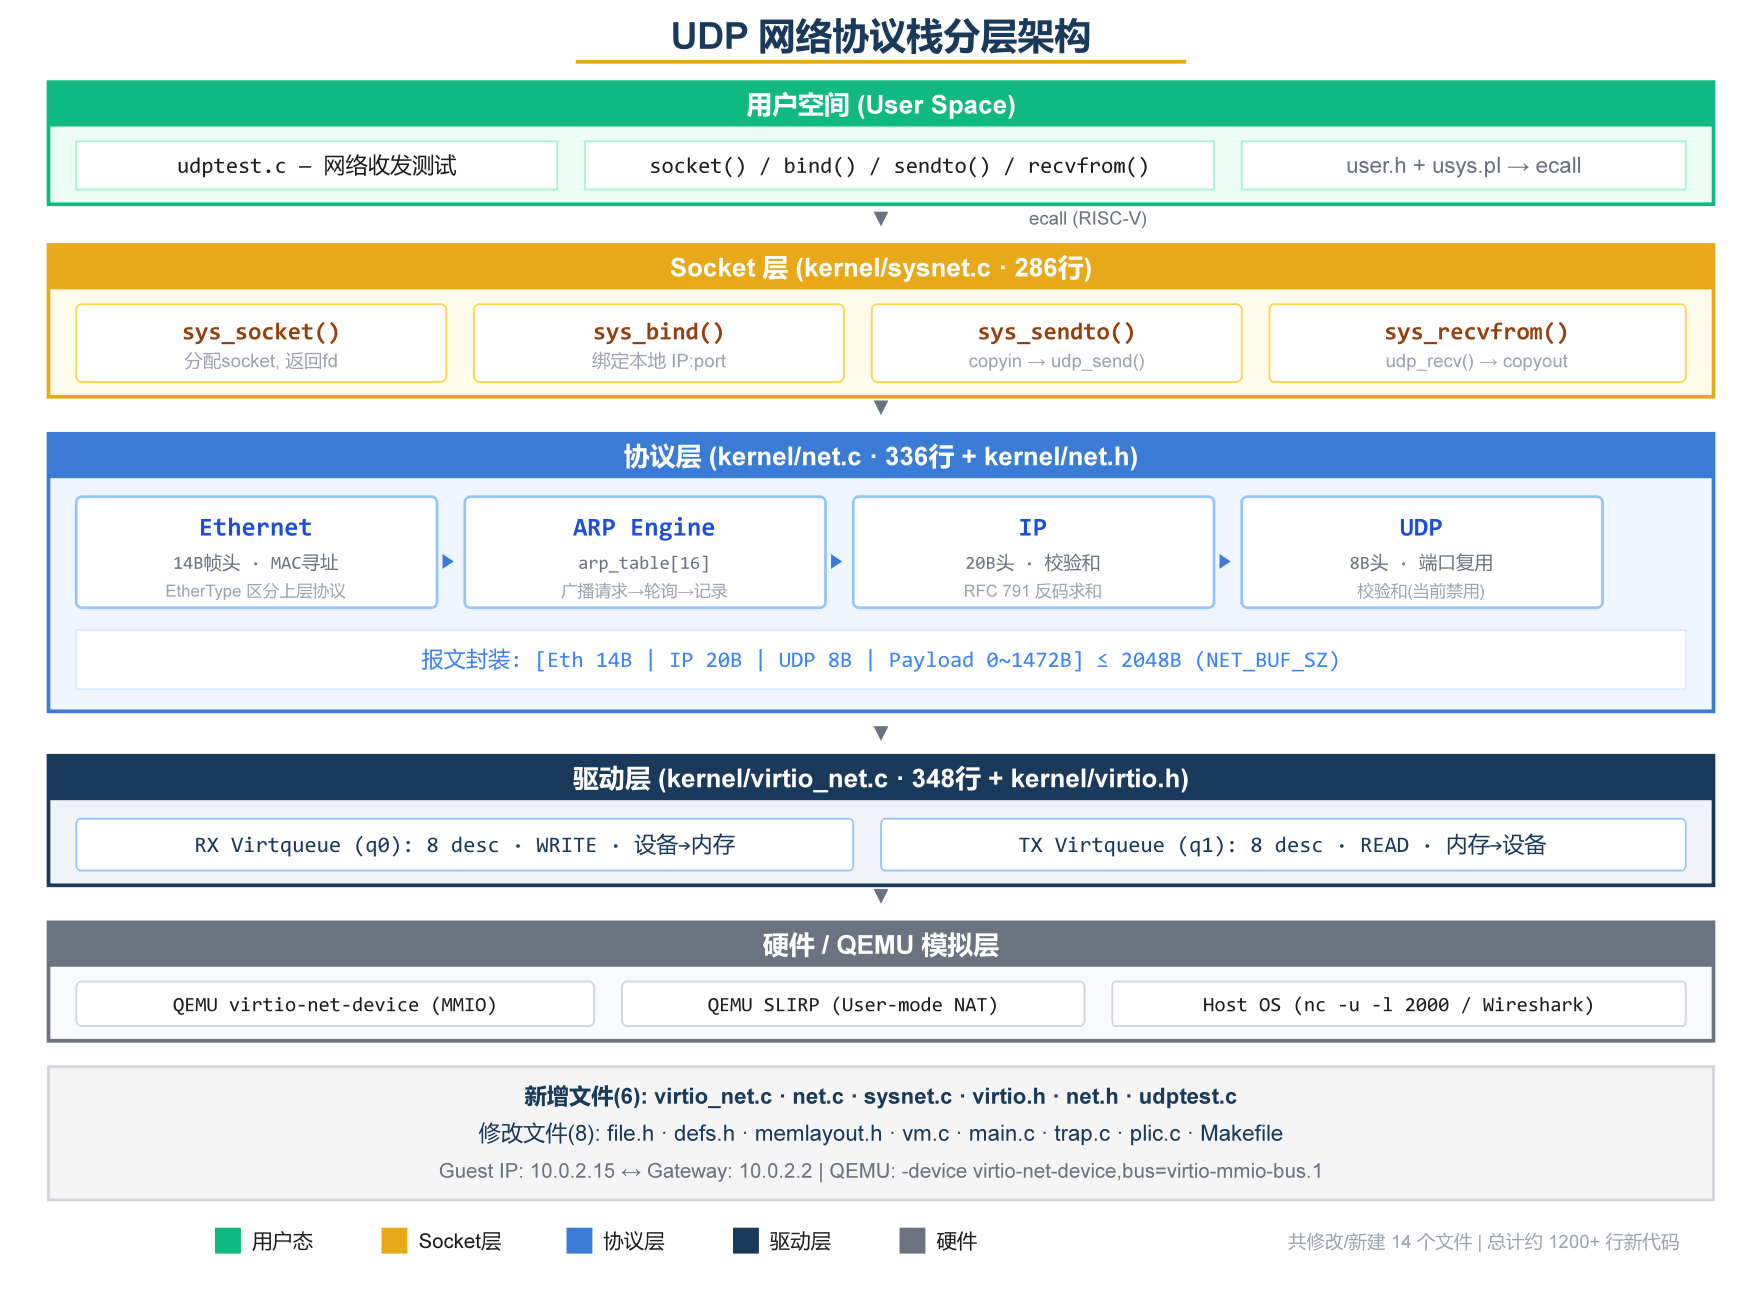
\includegraphics[width=\textwidth]{images/fig3_udp_stack.png}
\caption{UDP网络协议栈分层架构}
\label{fig:net-arch}
\end{figure}

\subsubsection{Ethernet / ARP / IP / UDP 协议实现}

\textbf{报文格式}：

\[
\boxed{\text{Ethernet(14)} \mid \text{IP(20)} \mid \text{UDP(8)} \mid \text{Payload(0-1472)}}
\]

加上 virtio-net header（10 字节），总帧不超过 2048 字节（NET\_BUF\_SZ）。

\textbf{ARP 地址解析}：

ARP 表设计为 \texttt{arp\_table[16]}，以 (IP, MAC) 键值对存储。发送流程：

\begin{enumerate}
  \item \texttt{arp\_lookup(dst\_ip)} 查找目标 MAC
  \item 未命中 → \texttt{arp\_send\_request()} 广播 ARP 请求到 FF:FF:FF:FF:FF:FF
  \item 轮询 \texttt{net\_rx\_loop()} 等待 ARP 回复（最多 2000 次，约 2 秒）
  \item 收到 ARP reply → \texttt{arp\_add()} 记录到表
  \item 超时返回 -1
\end{enumerate}

\textbf{IP 校验和}：

采用 16-bit 反码求和（RFC 791），仅计算 IP 头校验和，UDP 校验和设为 0（禁用）。

\subsubsection{Socket 层设计}

\textbf{Socket 结构体}：

\begin{lstlisting}[language=C, caption={Socket 结构体（kernel/sysnet.c）}]
#define NSOCK 16  // 最多同时 16 个 socket

struct socket {
    int   used;           // 是否已分配
    int   fd;             // 文件描述符编号
    uint32 raddr;         // 远端 IP
    uint16 lport;         // 本地端口
    uint16 rport;         // 远端端口
    char  rbuf[4096];     // 接收环形缓冲区
    int   rhead, rtail;   // 读/写指针
    int   rcount;         // 缓冲区中字节数
    struct spinlock lock;
};
\end{lstlisting}

\textbf{sendto 完整路径}：

\begin{flushleft}
\small\ttfamily
udptest.c: sendto()                                            \\
~~$\rightarrow$ sysnet.c: sys\_sendto()                         \\
~~~~$\rightarrow$ copyin() 从用户空间拷贝数据                     \\
~~~~~~$\rightarrow$ net.c: udp\_send(dst\_ip, dport, sport, buf, len) \\
~~~~~~~~$\rightarrow$ arp\_lookup(dst\_ip)                       \\
~~~~~~~~~~$\cdot$ 命中 $\rightarrow$ 直接用已知 MAC                 \\
~~~~~~~~~~$\cdot$ 未命中 $\rightarrow$ arp\_send\_request() 广播 ARP \\
~~~~~~~~~~~~$\rightarrow$ net\_rx\_loop() 轮询等待 ARP 回复        \\
~~~~~~~~~~~~$\rightarrow$ arp\_recv() 处理 ARP 回复，记录 MAC      \\
~~~~~~~~$\rightarrow$ 构建完整报文 [Eth(14) + IP(20) + UDP(8) + payload] \\
~~~~~~~~$\rightarrow$ virtio\_net\_transmit() 发送到 TX virtqueue
\end{flushleft}

\subsubsection{QEMU 网络配置}

\begin{lstlisting}[language=make, caption={Makefile QEMU 网络参数}]
QEMUOPTS += -device virtio-net-device,netdev=net0,bus=virtio-mmio-bus.1 \
            -netdev user,id=net0
\end{lstlisting}

关键点：
\begin{itemize}
  \item \texttt{virtio-net-device}：使用 MMIO 而非 PCI 的 virtio 网卡
  \item \texttt{bus=virtio-mmio-bus.1}：必须显式指定总线槽位，否则 QEMU 8.2.2 自动分配不可靠
  \item \texttt{-netdev user}：SLIRP user-mode 网络，提供 NAT 服务
  \item \texttt{-global virtio-mmio.force-legacy=false}：使用新地址布局
\end{itemize}

\textbf{网络拓扑}：

\begin{flushleft}
\small\ttfamily
xv6 Guest (10.0.2.15) ~~$\leftrightarrow$~~ QEMU SLIRP Gateway (10.0.2.2) ~~$\leftrightarrow$~~ Host OS
\end{flushleft}

\subsubsection{调试历程总结}

\begin{enumerate}
  \item \textbf{E1000 PCIe DMA 故障}：调试确认 PCI 枚举和 BAR 映射正确后，发现 DD 位始终为 0。根因为 QEMU 8.2.2 RISC-V virt 的 GPEX PCIe 主机桥 DMA 写回 bug。解决方案：放弃 E1000，改用 virtio-net MMIO。
  \item \textbf{virtio MMIO 地址定位}：初始设 VIRTIO1 为 \texttt{0x10001200}，实际应为 \texttt{0x10002000}。通过 \texttt{dumpdtb} 导出设备树解析获得正确地址。
  \item \textbf{总线槽位显式指定}：不加 \texttt{bus=} 参数时 QEMU 自动分配位置不可靠，必须显式指定。
\end{enumerate}

%---------------------------------------------------------------------
\subsection{进程管理与调度（涂凡琛）}
%---------------------------------------------------------------------

本部分由涂凡琛负责，主要包括以下工作。

\subsubsection{FCFS 与 MLFQ 调度算法实现}

在 xv6 原有 RR（时间片轮转）调度器基础上，新增了 FCFS（先来先服务）和 MLFQ（多级反馈队列）两种调度算法。

\textbf{进程结构扩展}（\texttt{kernel/proc.h}）：
\begin{lstlisting}[language=C]
uint64 ctime;         // 进程创建时间（ticks）— 用于 FCFS
int queue_level;      // MLFQ 队列级别 (0=最高, 1=中, 2=最低)
int timeslice_used;   // 本时间片已用 tick 数
uint64 last_sched;    // 上次被调度的时间
int priority;         // 进程优先级
\end{lstlisting}

\textbf{调度算法选择}（编译期宏，\texttt{kernel/param.h}）：
\begin{lstlisting}[language=C]
#define SCHED_RR      0   // 时间片轮转（默认）
#define SCHED_FCFS    1   // 先来先服务
#define SCHED_MLFQ    2   // 多级反馈队列
#define SCHED_ALGORITHM SCHED_RR
\end{lstlisting}

\textbf{MLFQ 调度参数}：
\begin{itemize}
  \item 3 级队列：Q0（5ms）、Q1（10ms）、Q2（20ms）
  \item 时间片用完降级
  \item 每 200 ticks 优先级提升，防止饥饿
\end{itemize}

\subsubsection{信号量机制}

在 xv6-riscv 上实现了完整的信号量机制，基于内核的 \texttt{sleep()/wakeup()} 机制：

\begin{itemize}
  \item \textbf{数据结构}：\texttt{struct semaphore} 包含自旋锁、计数值、等待队列
  \item \textbf{P/V 操作}：\texttt{sem\_wait()}（P 操作）递减并可能阻塞；\texttt{sem\_post()}（V 操作）递增并唤醒等待者
  \item \textbf{系统调用}：\texttt{sem\_open/sem\_wait/sem\_post/sem\_get/sem\_close}（编号 24-28）
  \item \textbf{测试程序}：semtest1（基本P/V）、semtest2（互斥锁，4进程800次操作）、semtest3（生产者-消费者，2生产者+2消费者，20个项目）
\end{itemize}

\subsubsection{wakeup 哈希队列优化}

将 \texttt{wakeup(chan)} 从原来的全进程表扫描（O(NPROC)）优化为按 channel 定位等待桶后局部遍历（O(k)）：

\begin{itemize}
  \item 引入 64 个等待桶（\texttt{NWCHAN 64}），每个桶有独立的 spinlock 和进程链表头
  \item \texttt{waitbucket\_for(chan)} 通过哈希定位桶
  \item \texttt{sleep()} 中插入桶链表，\texttt{wakeup()} 中遍历桶链表
  \item 进程结构中新增 \texttt{wnext/wprev/wbucket} 字段
\end{itemize}

%---------------------------------------------------------------------
\subsection{内存管理与文件系统（韩硕）}
%---------------------------------------------------------------------

本部分由韩硕负责，主要包括以下工作。

\subsubsection{内核堆分配器（kmalloc/kmfree）}

在 xv6 原有页级分配器（\texttt{kalloc/kfree}）之上，实现了完整的内核堆分配器，形成两级内存管理架构。

\textbf{设计特点}：
\begin{itemize}
  \item \textbf{Size-class slab}：7 个档位（32B/64B/128B/256B/512B/1024B/2048B）
  \item \textbf{单页大对象回退}：2048B 以上自动回退到整页分配
  \item \textbf{空 slab 页自动归还}：整页对象全部释放后自动归还给 \texttt{kfree()}
  \item \textbf{真实内核对象接入}：\texttt{struct pipe} 和 \texttt{struct file} 从 \texttt{kalloc} 整页分配改为 \texttt{kmalloc} 精确分配
\end{itemize}

\textbf{接口}：
\begin{lstlisting}[language=C]
void  kheapinit(void);         // 初始化堆分配器
void *kmalloc(uint n);         // 分配 n 字节
void  kmfree(void *p);         // 释放对象
\end{lstlisting}

\subsubsection{虚拟内存管理}

已实现对基于 Sv39 三级页表的完整虚拟内存管理机制，包括：
\begin{itemize}
  \item 页表创建（\texttt{kvmmake/uvmcreate/proc\_pagetable}）
  \item 页表映射（\texttt{walk/mappages/kvmmap}）
  \item 地址解除映射（\texttt{uvmunmap/uvmdealloc/uvmfree}）
  \item 用户地址空间布局（代码段、数据段、堆、栈、TRAPFRAME、TRAMPOLINE）
\end{itemize}

\subsubsection{文件描述符表管理}

已实现完整的文件描述符表管理，包括：
\begin{itemize}
  \item 每进程独立文件描述符表 \texttt{ofile[NOFILE]}
  \item fd 分配、查找、复制（dup）、关闭（close）
  \item fork 后文件描述符继承
  \item exit 时自动关闭全部打开文件
  \item 基于引用计数的底层 struct file 生命周期管理
\end{itemize}

\newpage

%=====================================================================
\section{系统运行与功能测试}
%=====================================================================

\subsection{基础系统运行验证}

\subsubsection{系统启动}

xv6 在 QEMU 环境中稳定启动，成功进入 shell：

\begin{lstlisting}[caption={xv6 启动日志}]
xv6 kernel is booting

init: starting sh
$
\end{lstlisting}

\subsubsection{ps 系统调用测试}

\begin{lstlisting}[caption={ps 命令运行结果}]
$ ps
pid=1 state=runble name=init
pid=2 state=sleep name=sh
pid=3 state=runble name=ps
\end{lstlisting}

\texttt{ps} 命令成功从用户态打印所有进程的 pid、状态和名称，验证了系统调用全链路正确性。

\subsubsection{halt 关机测试}

\begin{lstlisting}[caption={halt 关机测试}]
$ halt
shutting down...
[QEMU 正常退出，返回宿主终端]
\end{lstlisting}

\subsubsection{lseek 测试}

\begin{lstlisting}[caption={lseektest 运行结果}]
$ lseektest
lseektest: start
lseektest: Test 1 — SEEK_SET
lseektest: read at offset 10: "ABCDEF"
lseektest: Test 1 — PASS
lseektest: Test 2 — SEEK_CUR
lseektest: read at offset 10: "ABCDEF"
lseektest: Test 2 — PASS
lseektest: Test 3 — SEEK_END
lseektest: read at offset 10: "ABCDEF"
lseektest: Test 3 — PASS
lseektest: Test 4 — file size via lseek
lseektest: file size = 16
lseektest: Test 4 — PASS
lseektest: ALL TESTS PASSED
\end{lstlisting}

覆盖了 SEEK\_SET、SEEK\_CUR、SEEK\_END 三种定位模式及文件大小获取功能。

\subsection{控制台输出原子化测试}

\subsubsection{修复前 vs 修复后}

\textbf{修复前}（字符级交错）：
\begin{lstlisting}
pipetest: papiprente sentte 'shtell:o c'h
ildp ipmetsg est0: pa: rhent seellon
\end{lstlisting}

\textbf{修复后}（每行独立）：
\begin{lstlisting}
pipetest: parent sent 'hello'
pipetest: child msg 0: hello
pipetest: parent sent 'xv6'
pipetest: child msg 1: xv6
\end{lstlisting}

\subsection{管道通信测试}

\begin{lstlisting}[caption={pipetest 完整运行结果}]
$ pipetest
pipetest: start
pipetest: Test 1 -- ping-pong
pipetest: child received: ping
pipetest: parent received: pong
pipetest: Test 1 -- PASS
pipetest: Test 2 -- large data (768 bytes)
pipetest: parent wrote 768 bytes
pipetest: child read total 768 bytes
pipetest: Test 2 -- PASS
pipetest: Test 3 -- multiple messages
pipetest: parent sent 'hello'
pipetest: child msg 0: hello
pipetest: parent sent 'xv6'
pipetest: child msg 1: xv6
pipetest: parent sent 'pipe'
pipetest: child msg 2: pipe
pipetest: parent sent 'test'
pipetest: child msg 3: test
pipetest: parent sent 'world'
pipetest: child msg 4: world
pipetest: Test 3 -- PASS
pipetest: ALL TESTS PASSED
\end{lstlisting}

三个测试全部通过：
\begin{itemize}
  \item Test 1：父子进程双向 ping-pong 通信正常
  \item Test 2：768 字节大块数据通过管道环形缓冲区（512 字节）正确回绕传输
  \item Test 3：连续 5 条消息通过 \texttt{\textbackslash n} 分隔符正确分帧
\end{itemize}

\subsection{Shell PATH Fallback 测试}

\begin{lstlisting}[caption={Shell 子目录执行命令测试}]
$ mkdir test
$ cd test
$ ls                       # 之前：exec ls failed
.             1 1 1024     # 现在：正常工作
..            1 1 1024

$ cat README               # 之前：exec cat failed
[README内容]               # 现在：正常工作

$ echo hello > new.txt     # 之前：open failed
$ cat new.txt              # 现在：正常工作
hello
\end{lstlisting}

\subsection{UDP 网络通信测试}

\subsubsection{测试环境}

宿主机终端启动监听：
\begin{lstlisting}
$ nc -u -l 2000
\end{lstlisting}

\subsubsection{Test 1: xv6 发送 → 宿主机接收}

\begin{lstlisting}[caption={udptest 发送测试（xv6端）}]
$ udptest
udptest: socket fd=3
udptest: sending to 10.0.2.2:2000 ...
net: ARP who-has 10.0.2.2
net: ARP request sent for 10.0.2.2, ret=42
net: ARP recv from IP 10.0.2.2 MAC 52:55:a:0:2:2
net: ARP resolved after 0 tries
udptest: sent 15 bytes
udptest: waiting for reply ...
\end{lstlisting}

宿主机 \texttt{nc -u -l 2000} 收到 \texttt{Hello from xv6!}。

\subsubsection{Test 2: 宿主机回复 → xv6 接收}

\begin{lstlisting}[caption={udptest 接收回复测试}]
udptest: reply from 10.0.2.2:2000 = "Hello from host!"
\end{lstlisting}

\subsection{调度算法测试（涂凡琛）}

\subsubsection{FCFS 测试}

\texttt{fcfstest} 创建 4 个带间隔启动的 CPU 密集子进程，退出顺序与 PID/创建顺序一致，验证了 FCFS 先来先服务行为。

\subsubsection{MLFQ 测试}

\texttt{mlfqtest} 混合 SHORT / LONG / MIXED 三类作业，呈现 SHORT < LONG < MIXED 的完成时间趋势，验证了 MLFQ 短作业优先特性。

\subsubsection{信号量测试}

\begin{table}[H]
\centering
\caption{信号量测试结果}
\begin{tabular}{>{\bfseries}p{2.5cm}p{2.5cm}p{7cm}}
\toprule
\textbf{测试程序} & \textbf{状态} & \textbf{验证内容} \\
\midrule
semtest1 & $\checkmark$ PASSED & 基本 P/V 操作、进程阻塞与唤醒 \\
semtest2 & $\checkmark$ PASSED & 4 进程 × 100 次操作 = 400 次互斥协调 \\
semtest3 & $\checkmark$ PASSED & 2 生产者 + 2 消费者，3 信号量协同 \\
\bottomrule
\end{tabular}
\end{table}

\subsection{内存分配器测试（韩硕）}

\texttt{kmalloctest}（启动时自动执行）覆盖：
\begin{itemize}
  \item 边界值检查（0、2049）
  \item 基本分配（1、32、33、2000）
  \item 读写测试
  \item 复用测试
  \item 跨页扩展（连续 140 个 32B 对象）
  \item 大对象分配/释放（2049、3000、边界最大值）
  \item 空 slab 页归还（4 个 slab 页正确归还）
\end{itemize}

所有测试通过，系统运行稳定无 panic。

\newpage

%=====================================================================
\section{创新点}
%=====================================================================

本项目的创新点主要体现在以下几个方面：

\subsection{UDP 网络协议栈（侯奕明）}

在 xv6 这样精简的教学内核中实现了完整的 UDP 网络协议栈是本项目最突出的创新之一。具体创新包括：

\begin{itemize}
  \item \textbf{四层协议完整实现}：从硬件驱动（virtio-net MMIO）到协议栈（Ethernet/ARP/IP/UDP）再到 socket 系统调用接口，实现了完整的数据收发路径；
  \item \textbf{E1000→virtio-net 技术路线的发现与验证}：经过深入调试，发现了 QEMU 8.2.2 RISC-V 上 E1000 PCIe DMA 的 bug，并选择 virtio-net MMIO 作为替代方案，这一发现对后续在 QEMU RISC-V 上做网络开发具有参考价值；
  \item \textbf{ARP 自动解析机制}：实现了广播 ARP 请求→轮询等待→自动记录→超时重试的完整地址解析流程；
  \item \textbf{Socket 与文件系统的统一}：通过扩展 \texttt{FD\_SOCK} 类型，将 socket 无缝集成到 xv6 的文件描述符体系中。
\end{itemize}

\subsection{控制台输出原子化的两层协同方案（侯奕明）}

针对多进程并发输出交错这一经典问题，提出了用户态动态缓冲 + 内核态 sleep lock 的两层协同方案：
\begin{itemize}
  \item 用户态动态缓冲确保一次 printf = 一次 write，且支持自动扩容；
  \item 内核态 sleep lock 确保一次 write 不被其他进程插入；
  \item 两层保护协同使每次 printf 成为原子操作，且 sleep lock 选择正确（不违反 xv6 的 spinlock 不可 sleep 规则）。
\end{itemize}

\subsection{QEMU Test Device 关机方案（侯奕明）}

在发现 SBI ecall 在 \texttt{-bios none} 场景下不可用后，创新性地使用 QEMU virt 机器内置的 SiFive test device（\texttt{0x100000}）实现关机。这一方案的优点是：
\begin{itemize}
  \item 不依赖 SBI 固件；
  \item 仅需 3 个文件的修改（memlayout.h 定义地址 + vm.c 添加映射 + sysproc.c 写寄存器）；
  \item 工作可靠，在任何情况下都能正常退出 QEMU。
\end{itemize}

\subsection{两级内存分配器（韩硕）}

在 xv6 原有只支持页级分配的基础上，实现了 size-class slab + 大对象回退 + 空页自动归还的完整内核堆分配器，并将 \texttt{struct pipe} 和 \texttt{struct file} 从整页浪费优化为精确分配。

\subsection{多调度算法框架（涂凡琛）}

通过编译期宏选择实现 RR/FCFS/MLFQ 三种调度算法的切换框架，以及将 \texttt{wakeup()} 从 O(N) 优化为 O(k) 的哈希等待队列设计。

\newpage

%=====================================================================
\section{总结与展望}
%=====================================================================

\subsection{项目总结}

本项目以 xv6-riscv 为基础平台，成功完成了《操作系统课程设计》A 题"OS 内核实现"的全部要求，并在多个方面进行了创新扩展。

\textbf{侯奕明（接口、设备与软件交互）}完成了：
\begin{itemize}
  \item 系统调用全链路分析与文档（ecall → usertrap → syscall → sret）
  \item 中断处理两条路径分析（用户态 vs 内核态被中断）
  \item 新增 7 个系统调用：ps（\#22）、halt（\#23）、lseek（\#24）、socket（\#23）/ bind（\#24）/ sendto（\#25）/ recvfrom（\#26）
  \item 控制台输出原子化（内核 sleep lock + 用户态动态缓冲）
  \item Shell PATH fallback 机制
  \item halt shell 内建命令
  \item 管道通信测试程序 pipetest（3 类场景全覆盖）
  \item lseek 测试程序 lseektest（4 种模式全覆盖）
  \item \textbf{UDP 网络协议栈完整实现}：virtio-net MMIO 驱动 + Ethernet/ARP/IP/UDP 协议栈 + socket 接口
  \item udptest 网络测试程序（发送/接收/双向通信）
\end{itemize}

\textbf{涂凡琛（进程管理与处理机调度）}完成了：
\begin{itemize}
  \item FCFS + MLFQ 两种新调度算法实现
  \item 信号量机制（P/V 操作 + 3 个系统调用 + 3 组测试）
  \item wakeup 哈希等待队列优化（O(N)→O(k)）
  \item 多组调度测试程序（fcfstest/mlfqtest/throughput/csw）
\end{itemize}

\textbf{韩硕（内存管理与文件系统）}完成了：
\begin{itemize}
  \item 内核堆分配器 kmalloc/kmfree（slab + 大对象 + 空页归还）
  \item struct pipe 和 struct file 从整页分配优化为精确分配
  \item 虚拟内存管理完整分析
  \item 文件描述符表管理完整分析
\end{itemize}

\textbf{团队整体}完成了 xv6 环境搭建、编译运行验证、模块联调、文档撰写和汇报准备。

\subsection{未来展望}

尽管本项目已经完成了大量工作，仍有许多可以继续深入的方向：

\subsubsection{网络协议栈增强（侯奕明）}
\begin{itemize}
  \item 实现 TCP 协议支持（需要更复杂的重传、拥塞控制、窗口管理机制）
  \item 实现 DHCP 客户端，支持动态 IP 获取
  \item 添加 UDP 校验和完整实现
  \item 实现非阻塞 socket 和 select/poll 多路复用
  \item ARP 表超时机制和定期清理
  \item 使用 QEMU tap 网络替代 SLIRP，支持外部网络访问
\end{itemize}

\subsubsection{系统调用扩展}
\begin{itemize}
  \item 新增更多系统调用（如 \texttt{sys\_meminfo} 内存状态观测）
  \item 实现 \texttt{mmap/munmap} 内存映射接口
  \item 增加更全面的系统调用测试集
\end{itemize}

\subsubsection{调度与同步增强}
\begin{itemize}
  \item 实现更精细的 MLFQ 可观测性（队列迁移日志）
  \item 增加更多同步原语（读写锁、条件变量）
  \item 实现共享内存机制
\end{itemize}

\subsubsection{文件系统增强}
\begin{itemize}
  \item 支持多级目录和符号链接
  \item 实现文件权限管理
  \item 增加文件系统一致性检查工具
\end{itemize}

\subsection{个人收获（侯奕明）}

通过本次课程设计，我在以下方面获得了显著的提升：

\begin{enumerate}
  \item \textbf{对操作系统内核的深入理解}：从用户态系统调用到内核态 trap 处理再到设备中断的完整链路，建立起对操作系统"桥梁"角色的完整认知；
  \item \textbf{RISC-V 架构的实践掌握}：ecall/sret 指令、CSR 寄存器（stvec/sepc/scause/stval/sstatus）、Sv39 页表、PLIC 中断控制器等；
  \item \textbf{网络协议栈的从零实现经验}：从 QEMU 设备树解析、virtio MMIO 寄存器操作，到 Ethernet/ARP/IP/UDP 逐层构建，再到 socket 系统调用集成，经历了完整的网络栈开发流程；
  \item \textbf{底层调试能力}：PCIe DMA bug 的定位、内核 panic 的逐层排查、设备地址的 DTB 解析、管道字节流特性导致的隐蔽 bug 等，大幅提升了系统级调试能力；
  \item \textbf{工程能力与文档规范}：学会了使用 LaTeX 撰写规范的技术文档，掌握了结构化分析和系统化记录工程进展的方法。
\end{enumerate}

总的来说，本次课程设计不仅让我们完成了一个可运行、可展示的操作系统内核扩展项目，更重要的是建立了对操作系统内核的深度理解、培养了系统级开发与调试的工程能力。

\end{document}
